The magnetising field $H$ inside a solenoid is given by
\begin{equation}
    H = \frac{n I}{L}
    \label{H eqn}
\end{equation}
Where $n$ is the number of turns, $I$ the current, and L the solenoid length.
$\\$
This gives rise to the magnetic flux density $B$
For solenoids, with non-magnetic media in their core, there is a linear relationship:


\begin{align}
B &= \mu_0 (H + M) \\
M &= \chi H \quad \Rightarrow \quad B = \mu_0 (1 + \chi) H \\
\mu_r &= 1 + \chi \quad \Rightarrow \quad B = \mu_0 \mu_r H
\end{align}



However, when using magnetic materials, $\mu_r$ is not a constant and so:
\begin{equation}
    B = \mu_0 (H + M) 
\end{equation}
$\mu_0$ is the permeability of free space ($4\pi \times 10^{-7} \, \mathrm{H/m} \approx  1.257 \times 10^{-6} \, \mathrm{H/m}$),
$\\$
$\mu_r$ is the relative permeability of the material.
$\\$
$M$ is the magnetisation of the core material.
$\\$
$\chi$ is the volume magnetic susceptibility
$\\$
$\\$
By using different materials within the centre of the solenoid different values of $mu$ are used resulting in different hysteresis loops being formed.
These B and H values cannot be measured directly. But if you arrange 2 solenoids as in ($\textbf{\Cref{fig:transformer_coils}}$).

\begin{figure}[h]
    \centering
    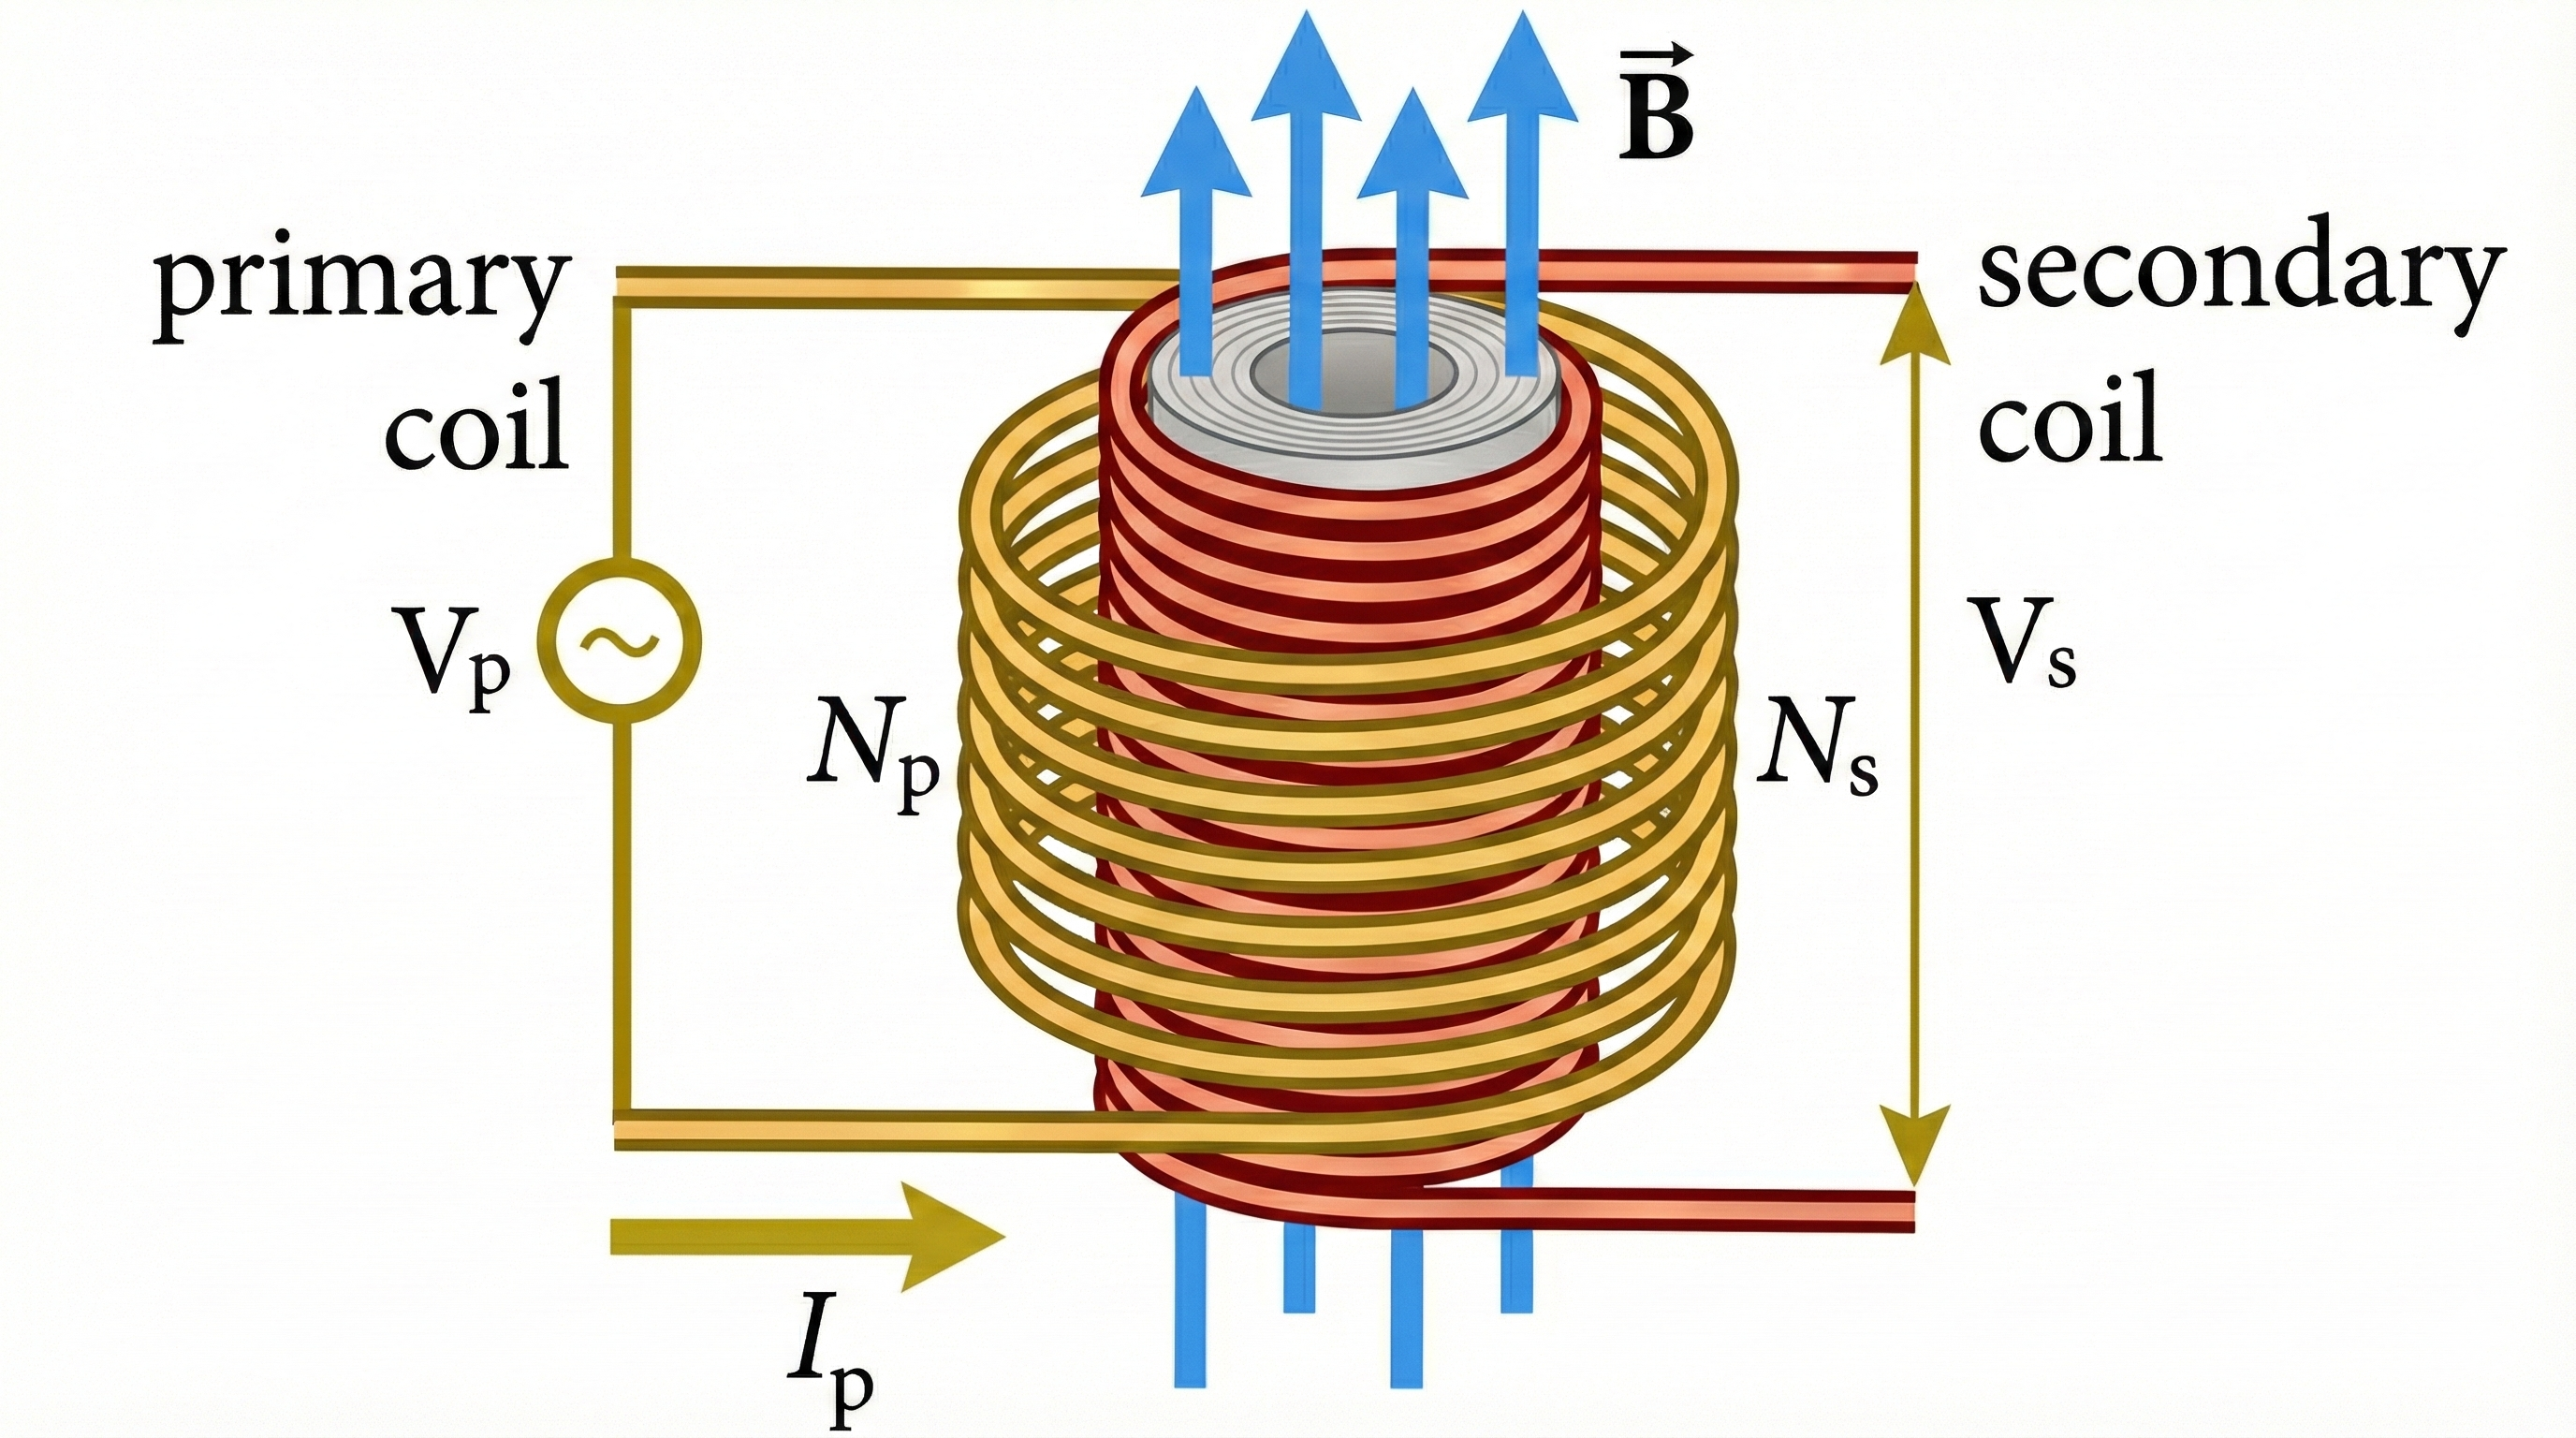
\includegraphics[width=0.5\textwidth]{../report/figures/transformer images 1.png}
    \caption{Interlinked solenoids \cite{transformer_coils}.}
    \label{fig:transformer_coils}
\end{figure}
$\\$
the variance of the magnetic field in one (the primary solenoid) results in an induced ${emf}$ in the other coil. This is given by Faraday's law of induction:

\begin{equation}
    \mathcal{E} = - N_s \frac{d\Phi}{dt}
\end{equation}
\noindent
Where:
\noindent
$\mathcal{E}$ is the ${emf}$ induced in the secondary coil
$N_s$ is the number of turns of coil
And $\frac{d\Phi}{dt}$ is the rate of change of flux
$\\$
\noindent
$\Phi$, the magnetic flux given by:

\begin{equation}
    \Phi = B A_s
\end{equation} 
\noindent
Where $B$ is the magnetic flux density inside the coil and is provided by the primary coil and $A_s$ is the area 
of the secondary coil.
$\\$
\noindent
$A_s$ is the Crossectional area of the material in the core.
$\\$
$\\$
This secondary coil then allows us to calculate $B$ by integrating $\mathcal{E} = - N_s \frac{d\Phi}{dt}$ to give:

\begin{equation}
    B = - \frac{1}{N_s A_s} \int \mathcal{E} dt
\end{equation}
$\\$
Then through the use of an integrator circuit we can let $V_{out} = -\frac {1}{R_i C} \int \mathcal{E} dt$ and then calculate B using: 
\begin{equation}
    B = - \frac {R_iC}{N_s A_s} V_{out}
\end{equation}
$\\$
\noindent
Our loop allows us to calculate the energy loss per cycle from the area under the $B$-$H$ curve and the $\mu_r$ 
values at different points. In this case, $\mu_r =\frac{1}{\mu_0} \frac{\partial B}{\partial H}$ as linear dependence is assumed in the localised region.
